
\noindent
This section analyses the behaviour of the best generative and evaluative models: V2 and V11 respectively. To perform this analysis we look at predictions on the DS2-Test set, which contains 124,137 grasps. %First, we would like to understand the statistics of the test data: how good are the grasps, are some grasps better than others? Second, we would like to know how well calibrated the evaluative model is, in other words we want to know how closely it predicts the grasp success probability. Third, we would like to know how much better the evaluative model is at ranking grasps than the initial ranking by the generative model. Finally, we want to how the evaluative model goes about improving performance, does it learn to re-rank grasp types or does it also do a good job of re-ranking grasps instances within a particular grasp-type?
%\subsection{How do grasp-type success rates vary?}
%\noindent
\begin{figure}[h]
\centering 
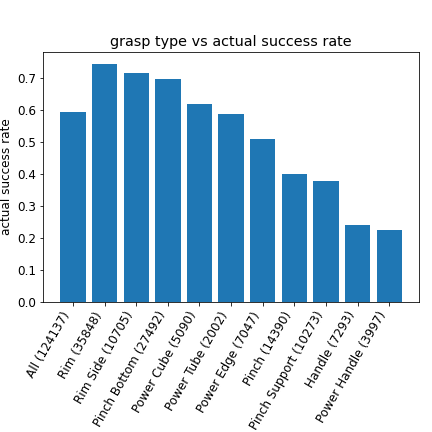
\includegraphics[width=0.5\columnwidth]{images/post-analysis/Grasp_type_vs_success_prob.png}
\caption{Grasp type vs. actual success rate.}
\label{fig:post2}
\end{figure}

%\subsection{How well are grasp success probabilities predicted?}
%\noindent
The first observation (Figure~\ref{fig:post2}) is that some grasp types are more likely to succeed than others. Grasp types with more finger links in contact with the object, such as Rim, Rim Side, or Power Cube have a higher success rate than those with fewer contacting links, such as Pinch and Handle.  This is due to the increased tolerance for finger positioning errors and the greater wrenches resisted when more contacts are made. 

The next question is how closely predicted success rates match the actual grasp success rates. Figure~\ref{fig:calibrate} is a histogram of successful (green) and unsuccessful (red) grasps in the test set. The historgram is organised on the horizontal axis by the predicted grasp success probability according to V11. The vertical axis shows the proportion of grasps that were actually successful. The closer the blue line is to the straight line showing perfect calibration, the better the prediction of the probability of success. When we aggregate all grasp-types, this prediction is close to perfect. The correlation also holds, though more weakly, when broken out across grasp types. \footnote{Where there is little data in the test set we plot the 95\% confidence interval for actual grasp success rate. Where the confidence interval is large we cannot draw a strong conclusion about the predictive power. The major deviations from perfect calibration are in areas with little data.}
%This suggests that V11 performance in the real robot experiments could be further improved by employing multiple views of the same object until a grasp is found where the network is highly confident that the grasp will succeed. Applying such an algorithm is beyond the scope of this paper, where the restrictions limits us to one view per object to generate grasps.

\begin{figure}[h]
\centering
\includegraphics[width=1.02\columnwidth]{images/post-analysis/V11_pred_success_vs_success.png}
\caption{Predicted success probability vs actual success probability for V11. The red bars indicate failures, and green bars show successes. The grasps are ordered along the horizontal axis by the predicted success probabilities of EM3. The blue line shows the (actual) average success rate of grasps in every bin, while the height of the shaded blue region is the standard error of the actual success rates in nearby bins. When there are insufficient grasps to estimate actual success rates (Handle and Power Tube), the uncertainty increases significantly.}
\label{fig:calibrate}
\end{figure}

%\subsection{How much better is the evaluative model's grasp ranking?}
%\noindent
The next question is how much better the evaluative model in V11 is than the generative model V2 in ranking grasps. The generative and evaluative models each produce a number for each grasp. This is a likelihood for the generative model (GM2) and a predicted probability of success for the evaluative model (EM3). These numbers are used to rank all the grasp-scene pairs in the test set. For a perfect ranking, all the successful grasps must be ranked above all the unsuccessful grasps. We can visualise the quality of each ranking using an ROC curve (Figure~\ref{fig:roc}). The metric used to compare different models is the area under the curve (AUC). It can be seen that V11 improves on V2 in separating successful from unsuccessful grasp instances for every grasp type. It also improves overall. The AUC across all grasps increases from 0.71 (V2) to 0.9 (V11). 

\begin{figure}[h]
\centering
\includegraphics[width=0.9\columnwidth]{images/post-analysis/V11_vs_v2_ROC_across_all_scenes}
\caption{\label{fig:roc}ROC curves for the evaluative model in V11 (EM3) and the underlying generative model (GM2/V2).}
\end{figure}

This analysis also shows that V11 successfully re-ranks grasps within a grasp type. Does the model also rank better than V2 between the grasp types? This can be answered by looking at the how much a method (V2 or V11) shifts up or down the average ranking of a grasp type relative to a random ranking. We calculate this shift for both V2 and V11 and then look at the correlation between this shift and the grasp-type success rate (Figure~\ref{fig:v2_vs_v11_rates}). This shows that both V2 and V11, on average, shift up grasp types that are more likely to be successful and shift down grasp types that are less likely to be successful. So, although the rankings are of grasp instances, we see that the effect is that information about the success rate of grasp types is also encoded. The Pearson correlation coefficient between V11's average improvement rates and success rates is 0.94, while V2's coefficient is 0.69. Finally, we can envision the entire table of success rates (given as the percentage of successful grasps) for the simulated test set, conditioned on grasp type and test object-pose pairs (Figure~\ref{fig:gop}). This informs us which grasp types are better suited to which object-pose pair. 

%V11, which combines the generative model GM2 with the evaluative model EM3, yields a substantial improvement over GM2's ranking, improving GM2's simulation top-grasp success rate from 79.05\% to 90.49\%, and real-world performance from 81.6\% to 87.8\%. We hypothesise that two main factors could contribute to this result. First, EM3 could be assigning high predicted success probabilities to grasp types that are generally successful, and low probabilities to those grasp types that fail often. Effectively, this would mean that a ranking based on EM3's predicted probabilities would simply be favouring grasp types that are, on average, more successful than others. Second, within each grasp type, EM3 may be learning which approach trajectories and hand/finger positions are more likely to be successful with respect to the object. The second hypothesis is more interesting. Such evidence would imply that the network is learning to associate the object's geometry with the approach trajectory and configuration. Below, we look for evidence to support both factors.

%\subsubsection{Does the evaluate model learn to rank grasp types?}
%\noindent

%\begin{figure}
%\centering
%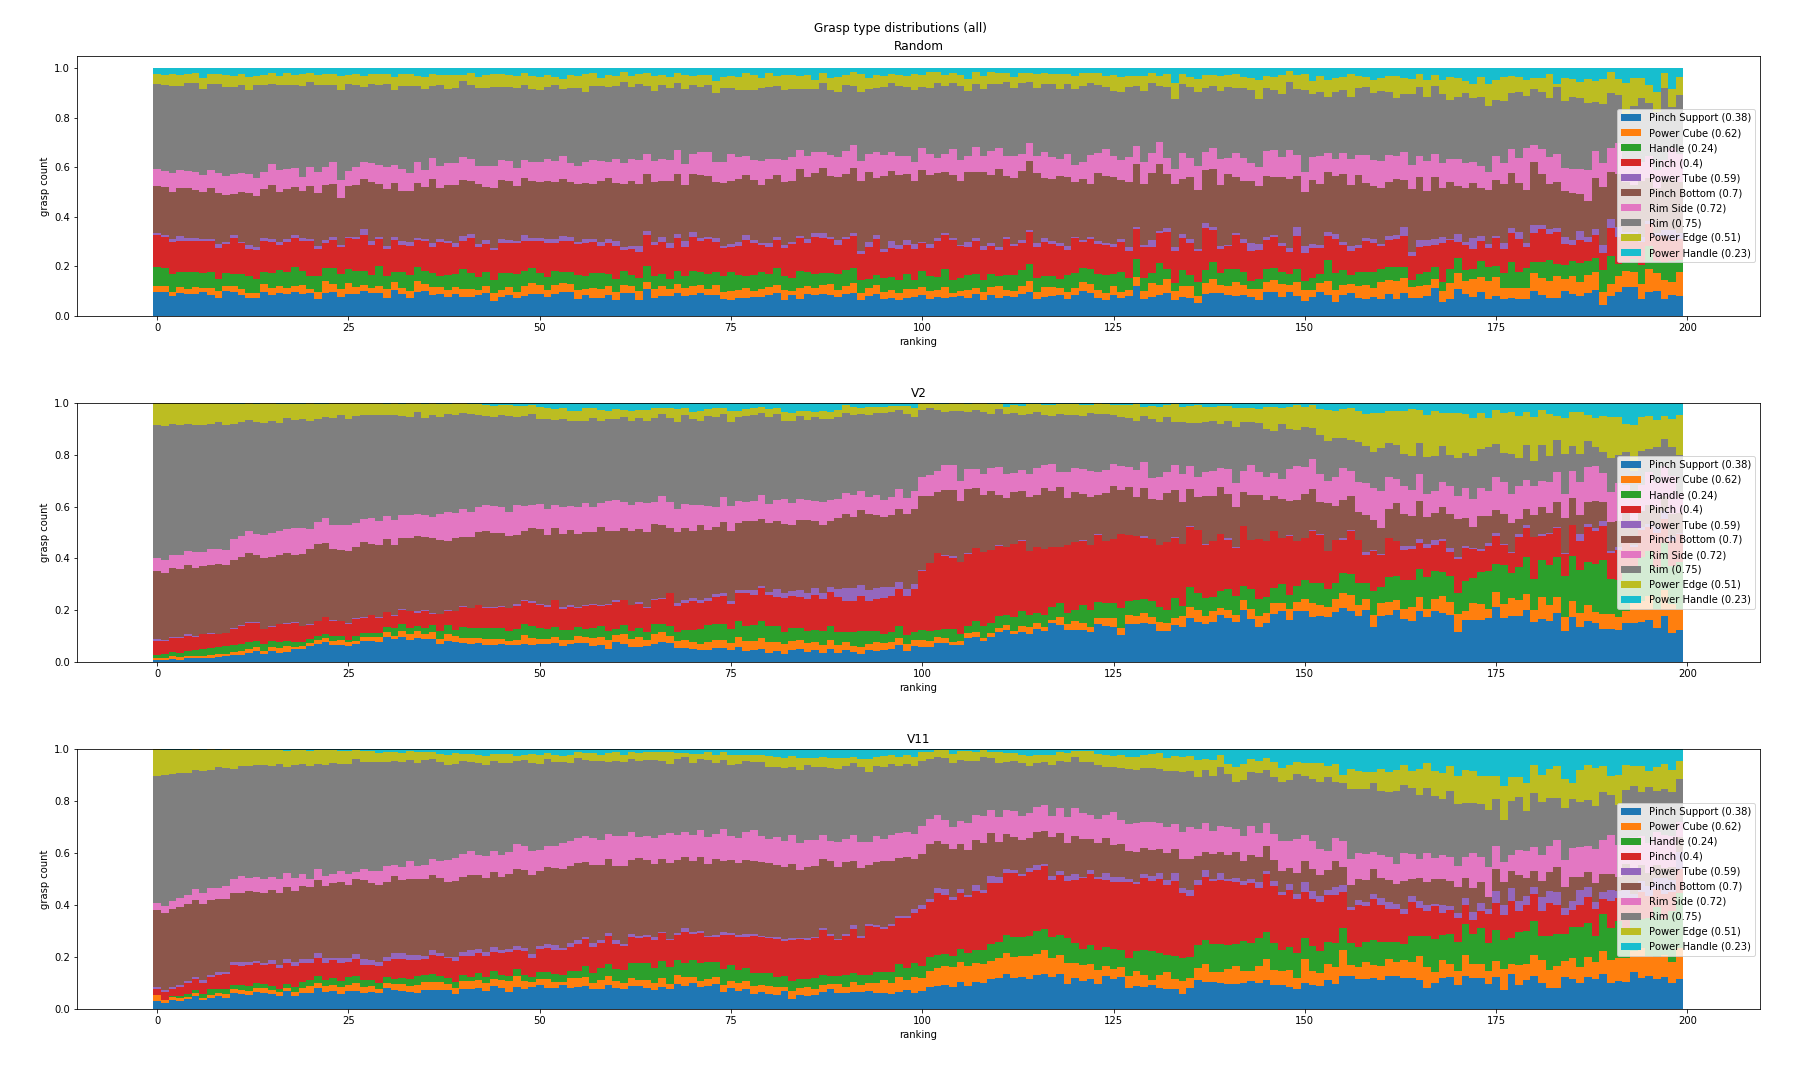
\includegraphics[width=0.8\columnwidth]{images/post-analysis/Grasp_type_distributions_all.png}
%\caption{Comparison of grasp type distributions per ranking of random, V2 and V11 rankings.}
%\label{fig:post6}
%\end{figure}

\begin{comment}
\begin{table}[h]
\small
\centering
\begin{tabular}{llll}
\hline
Grasp Type & Random Rank. & V2 Rank.  & V11 Rank.\\ \hline
Pinch Support & $\mathbf{97.4} \pm 82.8$  & $\mathbf{120.3} \pm 75.9 [\mathbf{+22.9}]$ & $\mathbf{111.9} \pm 78.6 [\mathbf{+14.5}]$ \\ \hline
Power Cube & $\mathbf{135.7} \pm 100.3$  & $\mathbf{162.4} \pm 92.1 [\mathbf{+26.7}]$ & $\mathbf{132.9} \pm 83.1 [\mathbf{-2.8}]$ \\ \hline
Handle & $\mathbf{97.2} \pm 83.3$  & $\mathbf{156.5} \pm 97.7 [\mathbf{+59.3}]$ & $\mathbf{149.5} \pm 86.2 [\mathbf{+52.3}]$ \\ \hline
Pinch & $\mathbf{87.1} \pm 72.7$  & $\mathbf{111.4} \pm 71.7 [\mathbf{+24.3}]$ & $\mathbf{104.5 }\pm 63.6 [\mathbf{+17.4}]$ \\ \hline
Power Tube & $\mathbf{121.0} \pm 92.5$  & $\mathbf{213.4} \pm 107.6 [\mathbf{+92.4}]$ & $\mathbf{118.7} \pm 82.6 [\mathbf{-2.3}]$ \\ \hline
Pinch Bottom & $\mathbf{89.8} \pm 69.5$  & $\mathbf{71.0} \pm 60.4 [\mathbf{-18.8}]$ & $\mathbf{75.6} \pm 77.9 [\mathbf{-14.2}]$ \\ \hline
Rim Side & $\mathbf{107.6} \pm 89.6$  & $\mathbf{91.6} \pm 69.2 [\mathbf{-16.0}]$ & $\mathbf{115.9} \pm 83.6 [\mathbf{+8.3}]$ \\ \hline
Rim & $\mathbf{85.9} \pm 76.5$  & $\mathbf{61.5} \pm 54.6 [\mathbf{-24.4}]$ & $\mathbf{66.3} \pm 60.8 [\mathbf{-19.6}]$ \\ \hline
Power Edge & $\mathbf{125.0} \pm 98.5$  & $\mathbf{102.9} \pm 81.7 [\mathbf{-22.1}]$ & $\mathbf{123.4} \pm 99.4 [\mathbf{-1.6}]$ \\ \hline
Power Handle & $\mathbf{121.0} \pm 95.7$  & $\mathbf{216.1} \pm 106.3 [\mathbf{+95.1}]$ & $\mathbf{184.5} \pm 99.1 [\mathbf{+63.5}]$ \\ \hline
\end{tabular}
\caption{Changes in average grasp position per grasp type according to Random, V2 and V11 rankings.}
\label{table:rankingchanges}
\end{table}
\end{comment}

\begin{figure*}[h]
\begin{center}
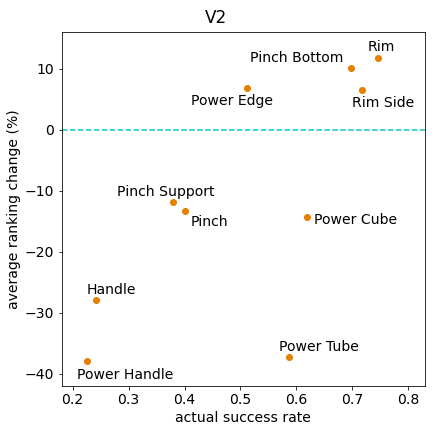
\includegraphics[width=0.35\textwidth]{images/post-analysis/V2_suc_rate_vs_improvement.png}~
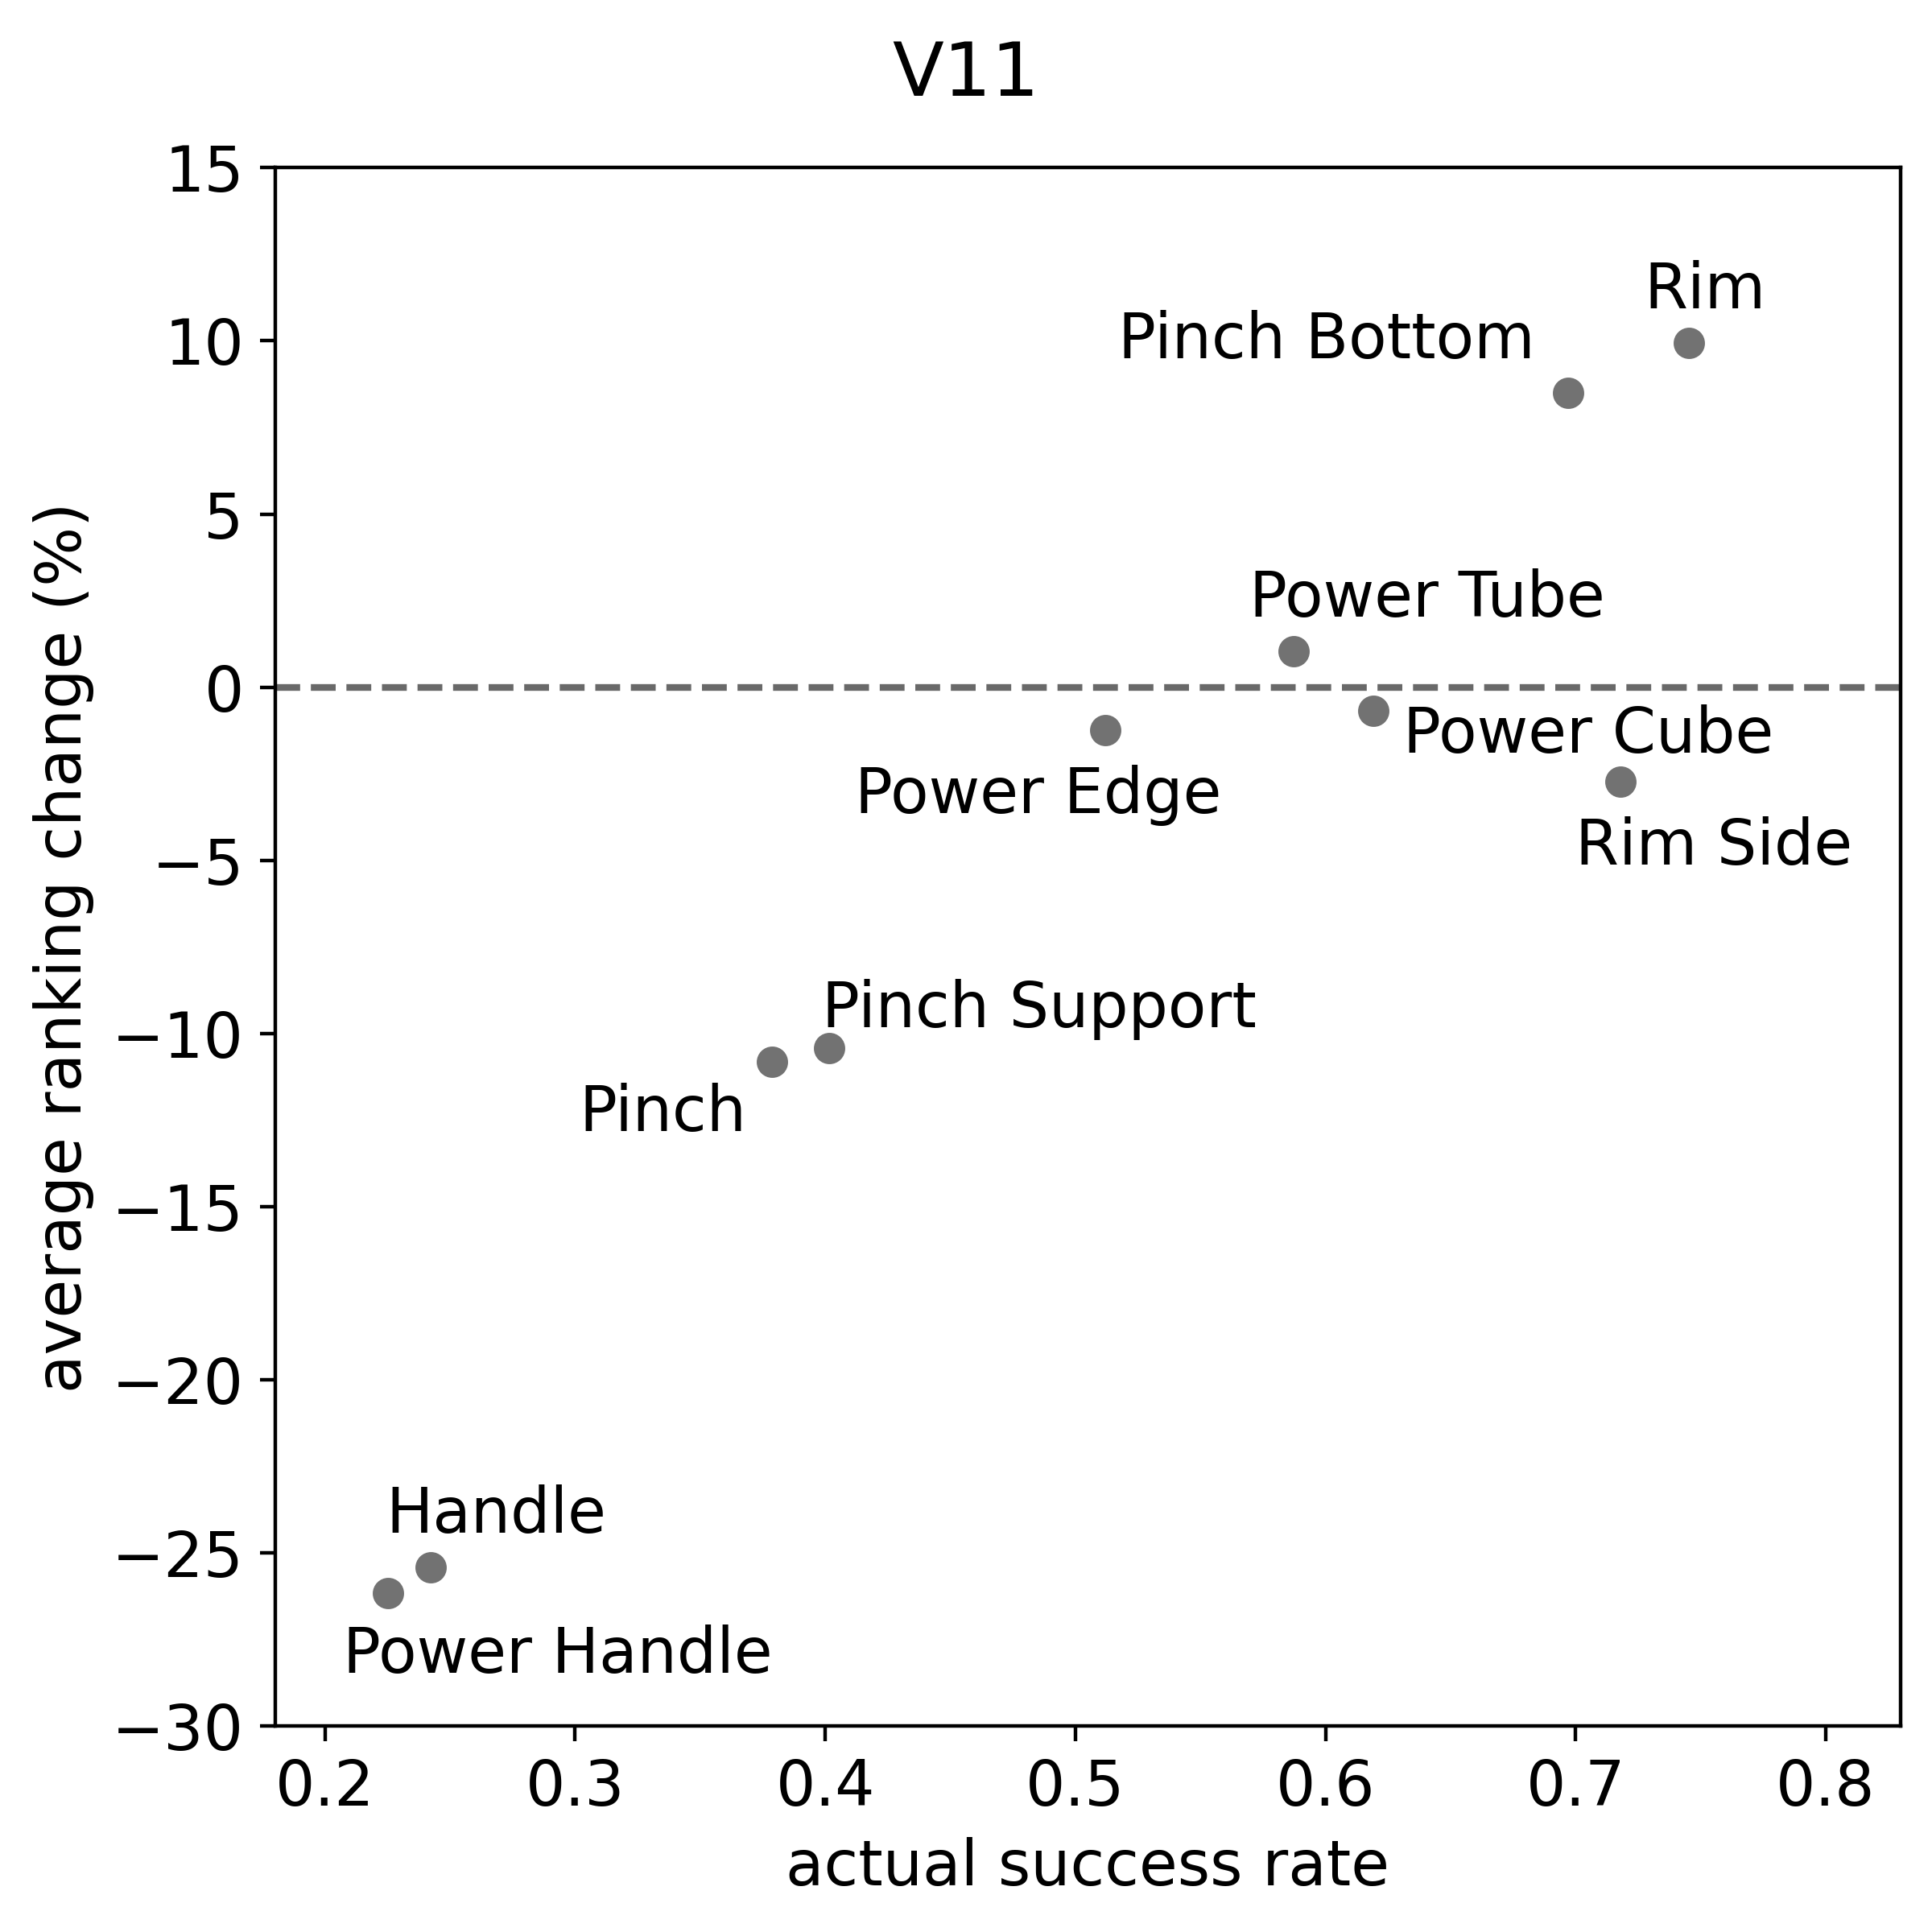
\includegraphics[width=0.35\textwidth]{images/post-analysis/V11_suc_rate_vs_improvement.png}
\caption{Comparing the per-grasp type average ranking improvement of V2 and V11, with random ranking taken as reference. Average ranking improvement is the average shift (\%) of all examples of a grasp type in a scene, aggregated across all test scenes where that grasp type is present. V11's shifts correlated with actual grasp success rates yield a Pearson coefficient of 0.94, while V2 achieves 0.69. \label{fig:v2_vs_v11_rates}}
\end{center}
\end{figure*}

\begin{figure}[h]
\centering
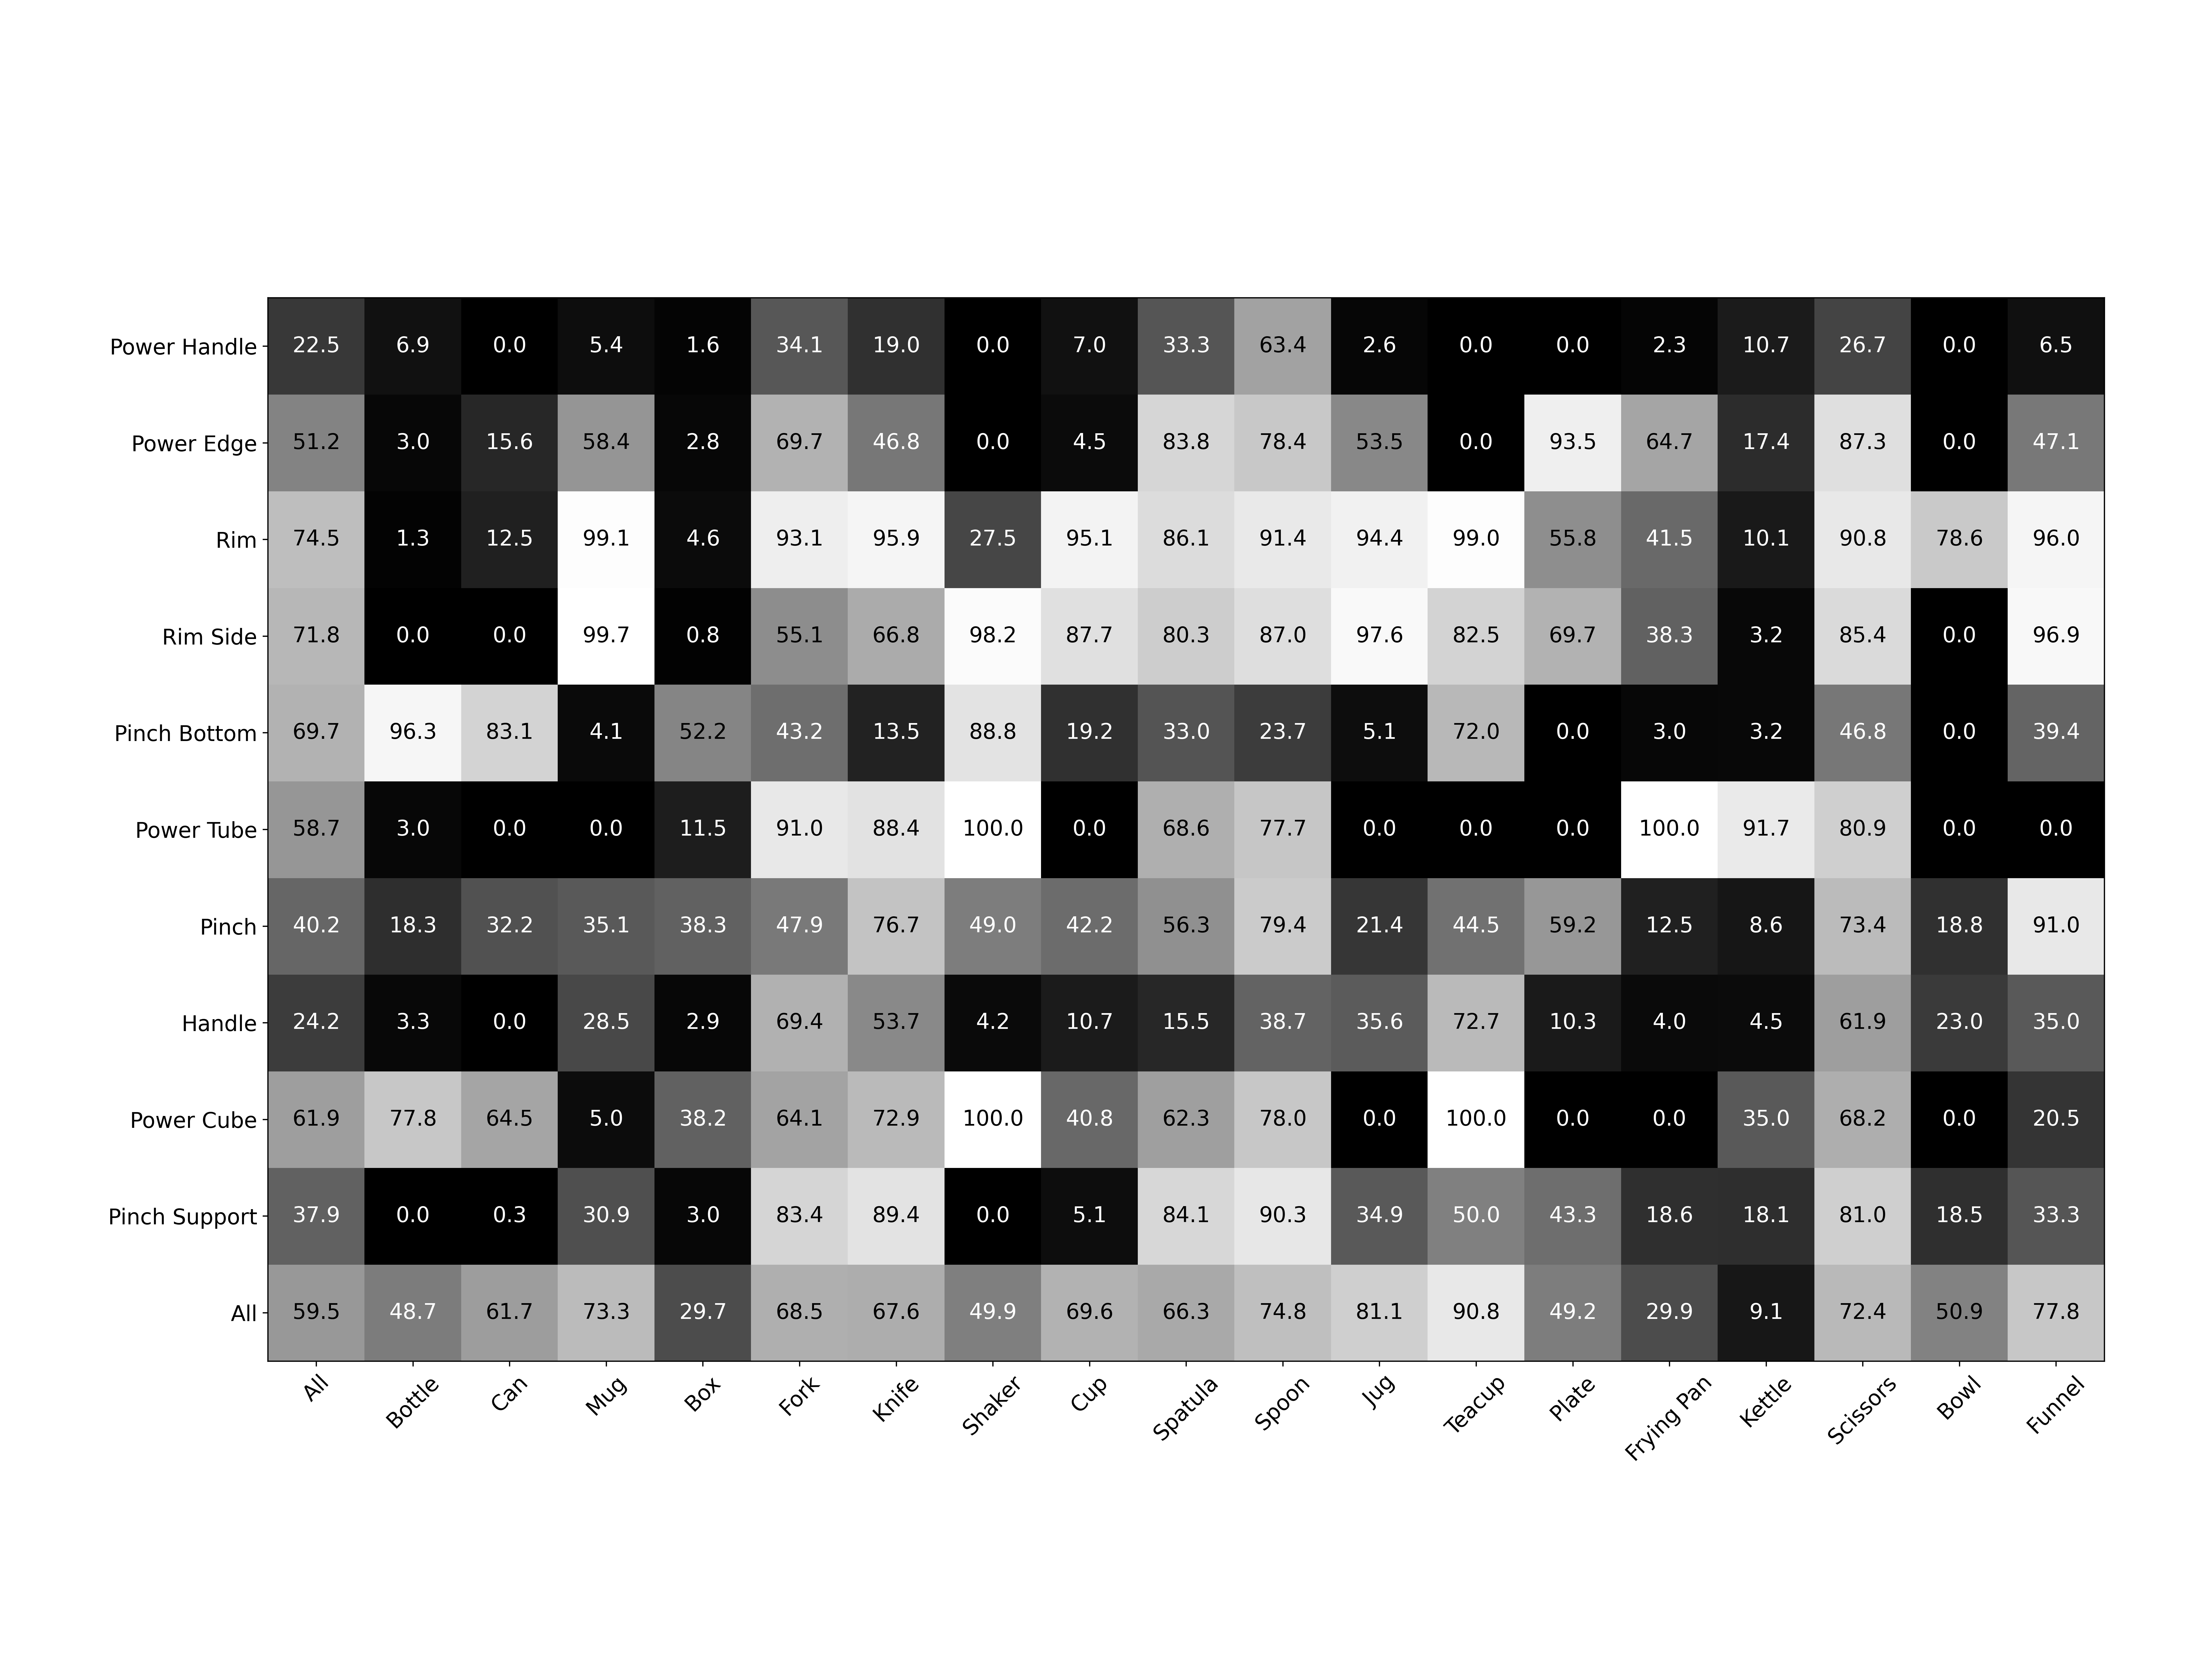
\includegraphics[width=\columnwidth]{images/mean_success_rate_per_grasp_type_and_object_class}
\caption{\label{fig:gop} Success rate, as a percentage, for each grasp type and object-pose pair in the simulation test set.}
\end{figure}
%Figure~\ref{fig:v2_vs_v11_rates} compares the per-grasp type average ranking improvement of V2, which is based on the generative model GM2, and V11, which employs evaluative model EM3. Both are calculated by taking the random ranking, which are based on randomly assigned success probabilities, as reference. Both V2 and V11 appear to favour robust grasps over that fail more often, despite calculating the grasp success probabilities in entirely different ways. The Pearson correlation coefficient between V11's average improvement rates and actual success rates is 0.94, while V2's coefficient is only 0.69. While a causal link is yet to be established, V11 ranking's strong correlation with per-grasp-type success rates suggests V11 (therefore EM3) learns to rank grasps according to their grasp types.

%\begin{figure}
%\centering
%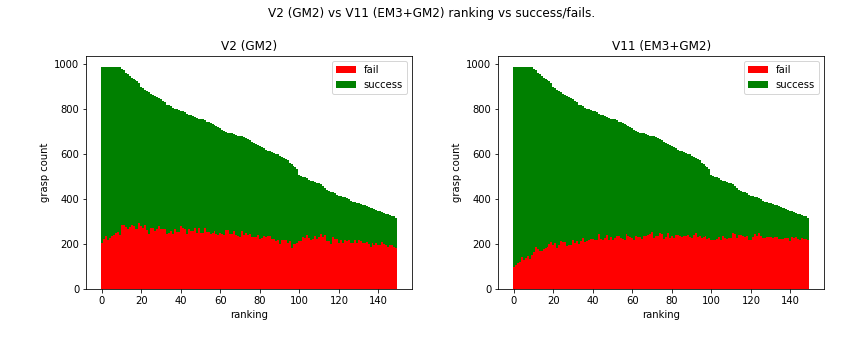
\includegraphics[width=0.8\columnwidth]{images/post-analysis/[3] V2_vs_V11_ranking_vs_success_fail.png}
%\caption{Comparison of successful (green) and unsuccessful (red) grasps per ranking for V2 and V11.}
%\label{fig:post3}
%\end{figure}

%\subsubsection{Does EM3 rank grasps within a grasp type?}
%\noindent

%The second hypothesis we have is that EM3 is learning to rank grasps within each grasp type, favouring grasp trajectories that are more likely to be successful over others. In order to test this hypothesis, we compared three different strategies above: random, V2, V11. In Figure~\ref{fig:post5}, we compare the the quality of the ranking of grasps within each grasp type. In order to compare rankings, a grasp's ranking, multiplied by -1, is used as the classification score in a binary classification problem (failure/success). The metric used to compare different models is the area under Receiver Operating Characteristics (ROC) curve. This metric is calculated for each scene, and averaged across all scenes in the test set. The left-most plot in Figure~\ref{fig:post5} shows that the overall ranking quality of V11 is better than V2 and random predictions across grasp types. Furthermore, V11 has the best overall within-type ranking for all grasp types except for Power Tube. This observation suggests that V11 not only leans on the grasp type information, but also learns to associate the object's geometry with the grasp trajectories to determine whether a grasp will be successful.

%\begin{figure}[h]
%\centering
%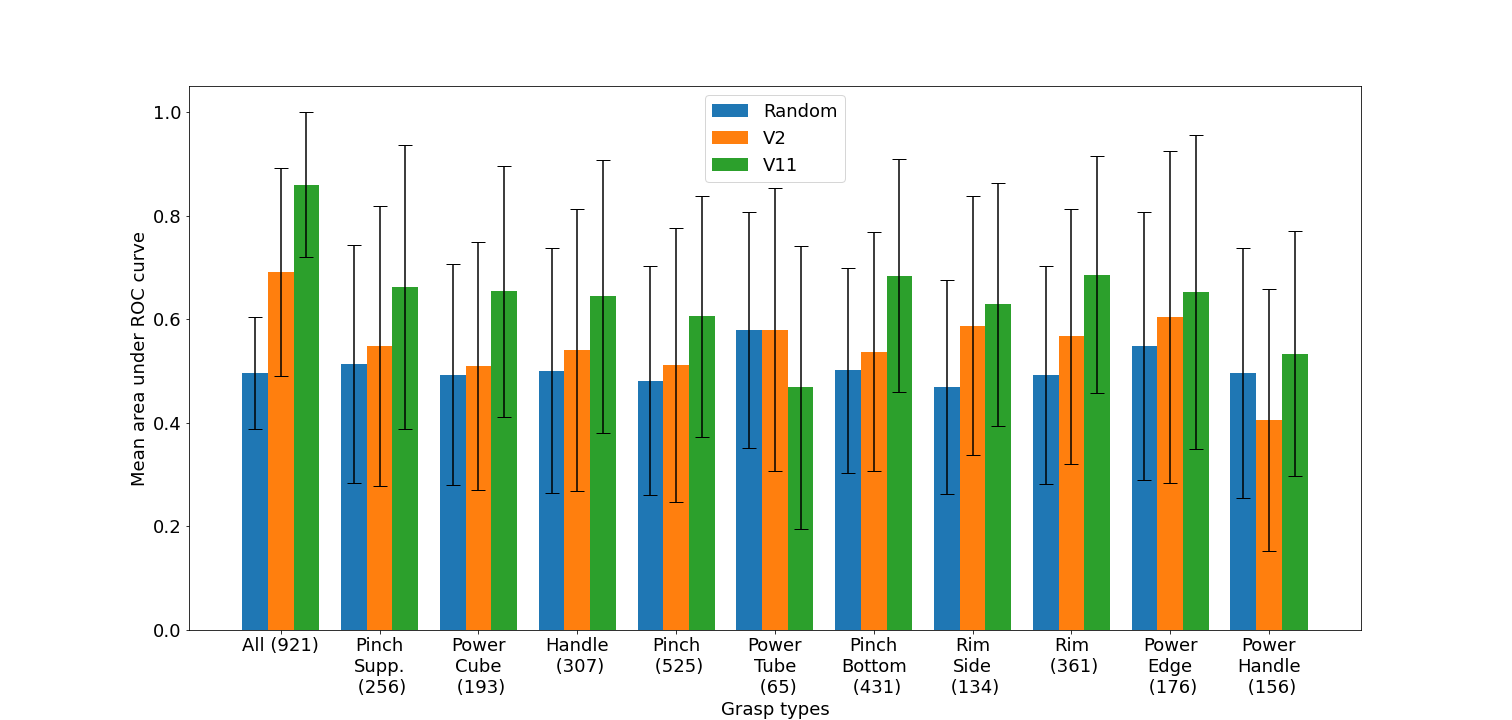
\includegraphics[width=0.999\columnwidth]{images/post-analysis/Ranking_quality_mean_AUC.png}
%\caption{Within-type grasp ranking quality comparison of random, V2 and V11 predictions according to the Area-Under-Curve of Receiver Operating Characteristics (AUC-ROC) metric. Higher score is better. V11's ranking outperforms those of random and V2, except for Power Tube.}
%\label{fig:post5}
%\end{figure}

%\begin{figure}
%\centering
%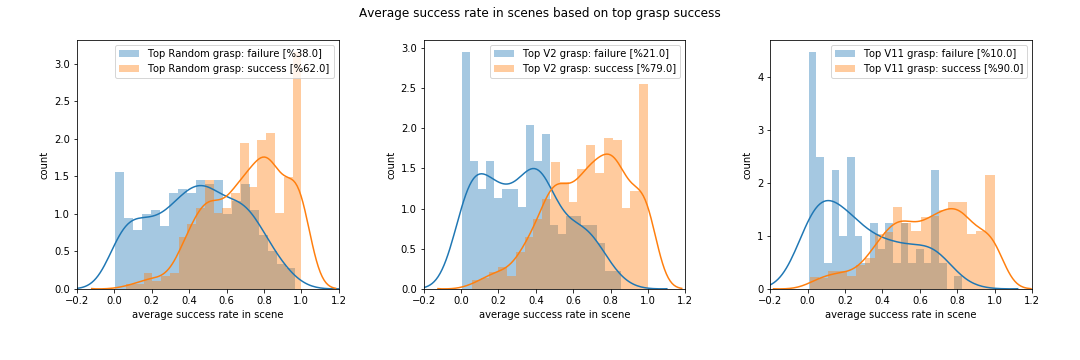
\includegraphics[width=0.8\columnwidth]{images/post-analysis/Average_success_rate_in_scenes_based_on_top_grasp_success.png}
%\caption{Average success rate in scenes vs top grasp success.}
%\label{fig:post7}
%\end{figure}

%\begin{figure}
%\centering
%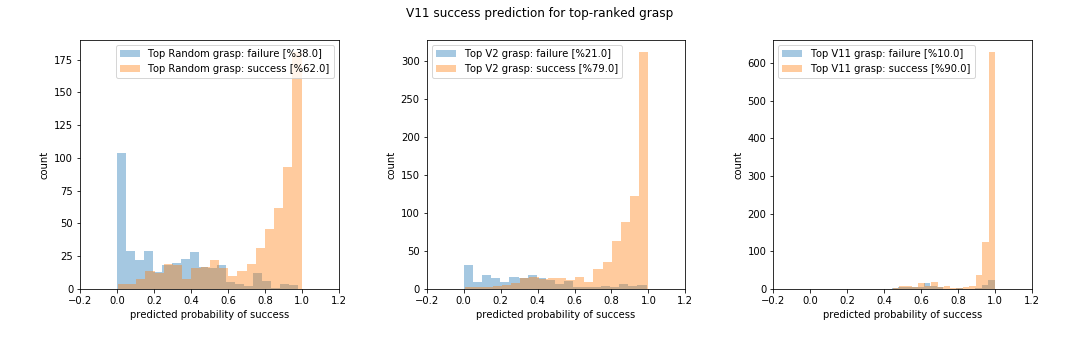
\includegraphics[width=0.8\columnwidth]{images/post-analysis/V11_success_prediction_for_top-ranked_grasp.png}
%\caption{Histogram of success rate of a top-ranked grasp vs its probability of success as estimated by V11.}
%\label{fig:post8}
%\end{figure}

%\begin{figure}
%\centering
%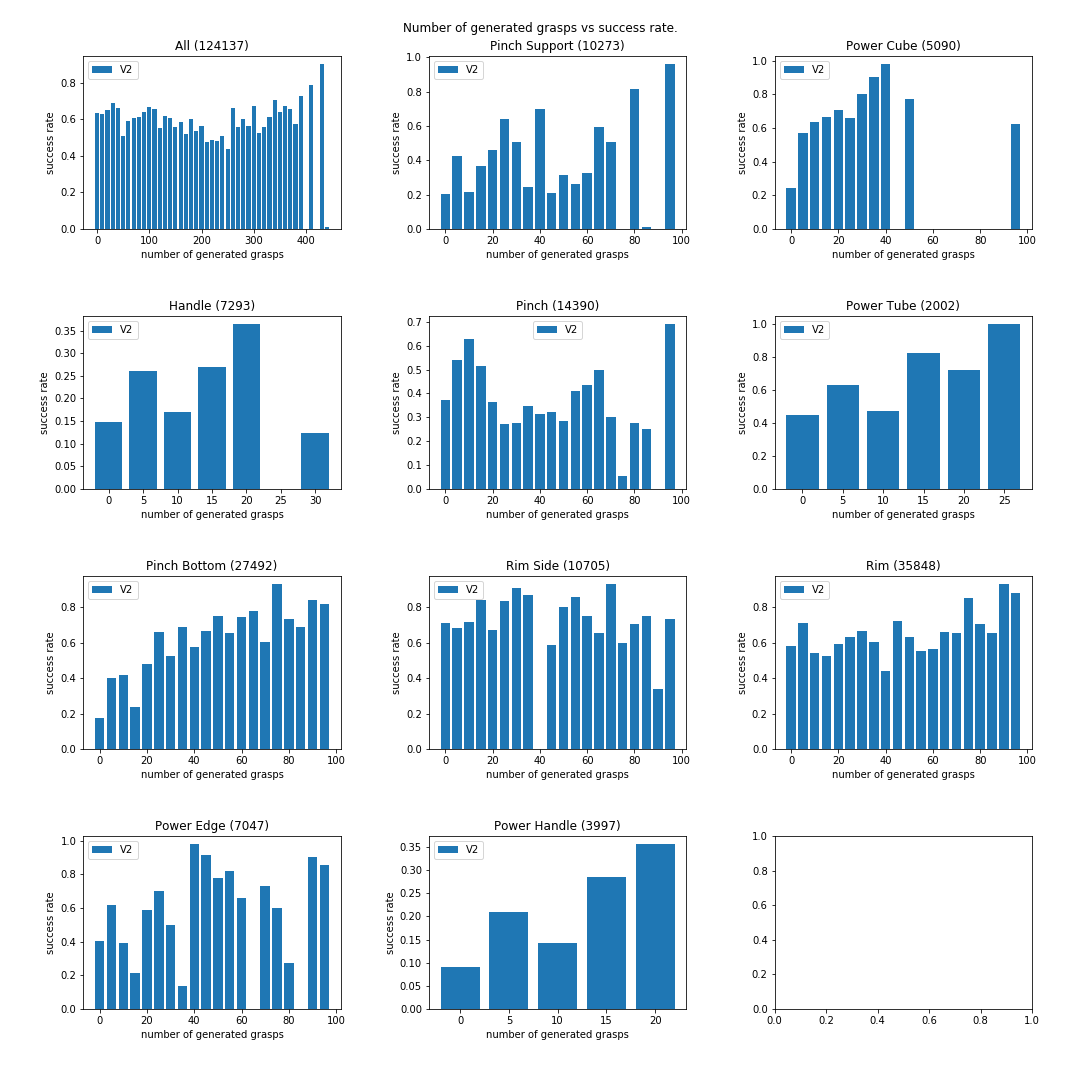
\includegraphics[width=0.8\columnwidth]{images/post-analysis/number_of_generated_grasps_vs_success_rate.png}
%\caption{Correlation of success rate with number of generated grasps per scene per grasp type.}
%\label{fig:post10}
%\end{figure}


%We compared the EM and GM rankings (Figure~\ref{fig:successvsranking}). The x-axis shows the ranking. The y-axis shows the average actual success rate over all scenes (1,241 test, 7,311 training). When ranked by the EM, the grasp success probability falls nearly monotonically, as is desirable. On the other hand, the likelihood-based ranking of GM results in many good grasps being low-ranked. We also wish to know whether the grasps recommended by the EM and the GM have different grasp success rates. The success rates of the top-ranked grasps are 71.59\% (GM) and  84.2\% (EM).

%A pure generative model architecture (GM) and the generative-evaluative architecture (GEA) were evaluated using a paired trials methodology. Each was presented with the same object-pose combinations. Each architecture generated a ranked list of grasps, and the highest ranked grasp was executed. The highest-ranked grasp based on the predicted success probability of the network is performed on each scene. A grasp was deemed successful if, when lifted for five seconds, the object then remained stable in the hand for a further five seconds before being automatically released. The success rate for GM was 57.1\% and for GEA it was 77.6\%. The successes and failures for each method were recorded and are summarised in Table~\ref{tab:robot-results}. A two-tailed McNemar test, for the difference between success rates for paired comparison data, was performed and the difference between the two algorithms has a $p$-value of 0.0442, and so is statistically significant. A selection of grasps where the two methods performed differently are shown in Figure~\ref{fig:successfail}.

% OLD TABLE
%\begin{table}
%\begin{center}
%\caption{Results of the real robot paired comparison trial.}
%\begin{tabular}{|c|c|c|c|}  \hline 
%          &                & \multicolumn{2}{ c |}{ GM} \\ \hline
%          &                & \# succs & \# fails  \\  \hline
 %GEA  & \# succs &  23 &  15  \\
 %         & \# fails    &  5   &   6   \\ \hline
%\end{tabular}
%\end{center}
%\label{tab:robot-results}
%\end{table}

%Training parameters for network. Training of example grasps for learning from demonstration. Creation of real test data set. Paired comparisons methodology with vanilla LFD algorithm (pose + object + camera view).
%
%The actual grasping tests have been performed on the real robot. 